\documentclass[10pt,border=5pt]{standalone}
\usepackage[T1]{fontenc}
\usepackage{lmodern,amsmath,amssymb,mathrsfs,tikz}
\usetikzlibrary{arrows.meta,positioning,calc}
\definecolor{ink}{HTML}{192536}
\definecolor{blue}{HTML}{2E70AE}
\definecolor{gold}{HTML}{A66A15}
\definecolor{green}{HTML}{28764D}
\definecolor{red}{HTML}{B43D3D}
\newcommand{\C}{\mathbb C}
\newcommand{\R}{\mathcal R}
\newcommand{\Lr}{\mathcal L_{\mathrm{res}}}
\newcommand{\Prs}{\mathcal P_{\mathrm{res}}}
\newcommand{\Tr}{T_{\mathrm{resp}}}
\newcommand{\rr}{\rho_{\mathrm{res}}}
\tikzset{every node/.style={font=\small,text=ink,align=center},
 box/.style={draw=blue,fill=blue!4,rounded corners=3pt,line width=.7pt,inner sep=7pt},
 goldbox/.style={box,draw=gold,fill=gold!5},
 greenbox/.style={box,draw=green,fill=green!5},
 redbox/.style={box,draw=red,fill=red!4},
 edge/.style={-{Stealth[length=4pt]},draw=ink,line width=.7pt},
 heading/.style={font=\small\bfseries},
 note/.style={font=\small,text=ink!85}}

\begin{document}
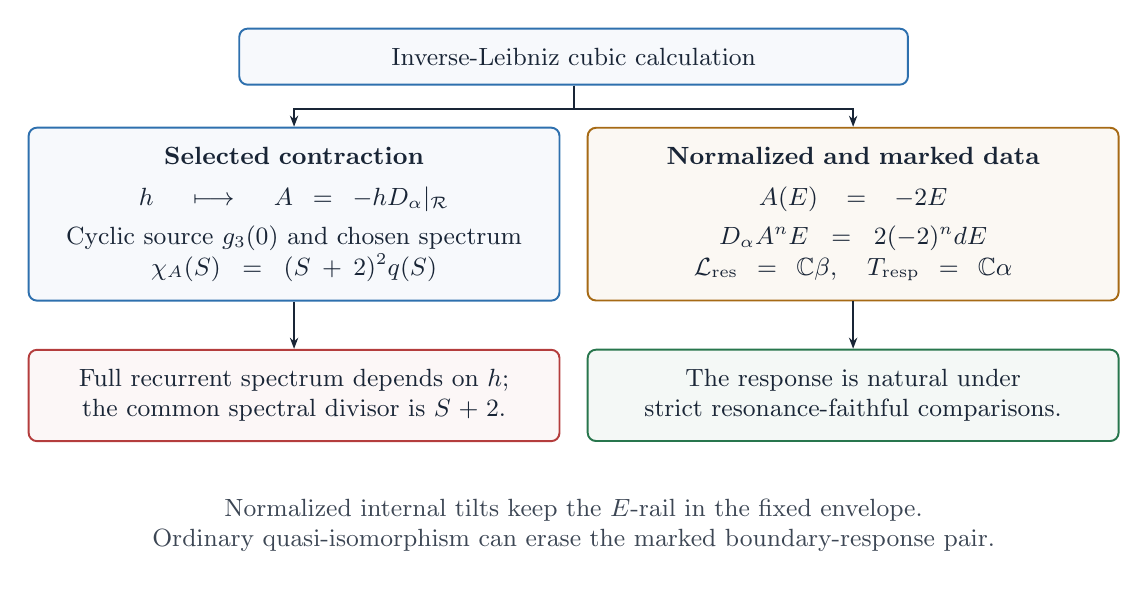
\begin{tikzpicture}
\node[box,text width=8cm] (root) {Inverse-Leibniz cubic calculation};
\node[box,text width=6.25cm] (chosen) at (-3.55,-2.0)
 {\textbf{Selected contraction}\\[4pt]
 $h\;\longmapsto\; A=-hD_\alpha|_{\R}$\\[3pt]
 Cyclic source $g_3(0)$ and chosen spectrum\\
 $\chi_A(S)=(S+2)^2q(S)$};
\node[goldbox,text width=6.25cm] (marked) at (3.55,-2.0)
 {\textbf{Normalized and marked data}\\[4pt]
 $A(E)=-2E$\\[3pt]
 $D_\alpha A^nE=2(-2)^n dE$\\
 $\Lr=\C\beta,\quad \Tr=\C\alpha$};
\draw[edge] (root.south) -- ++(0,-3mm) -| (chosen.north);
\draw[edge] (root.south) -- ++(0,-3mm) -| (marked.north);
\node[redbox,text width=6.25cm,below=6mm of chosen] (no)
 {Full recurrent spectrum depends on $h$;\\
 the common spectral divisor is $S+2$.};
\node[greenbox,text width=6.25cm,below=6mm of marked] (yes)
 {The response is natural under\\strict resonance-faithful comparisons.};
\draw[edge] (chosen) -- (no);
\draw[edge] (marked) -- (yes);
\node[note,text width=13.5cm,below=6mm of $(no.south)!0.5!(yes.south)$]
 {Normalized internal tilts keep the $E$-rail in the fixed envelope.\\
 Ordinary quasi-isomorphism can erase the marked boundary-response pair.};
\end{tikzpicture}
\end{document}
